\documentclass[a4paper]{article}
\usepackage{url}
\usepackage{graphicx}
\usepackage{enumitem}
\usepackage{xcolor}
\usepackage{amsmath}
\usepackage[vlined,noresetcount]{algorithm2e}
\usepackage{tikz}
\usepackage{float}
\usepackage{amssymb}
\usepackage[dvipsnames]{xcolor}
% \usepackage{amsthm}
% \theoremstyle{definition}
% \newtheorem{definition}{Definition}[section]
\usepackage{fancyhdr}
\pagestyle{fancy}
\fancyhf{}
\fancyhead[L]{\rightmark}
\fancyhead[R]{\thepage}
\renewcommand{\headrulewidth}{0pt}

\usepackage{pgfplots} 
\pgfplotsset{width=10cm,compat=1.9}

% \usepackage{csvsimple}
% \usepackage{longtable}
\usepackage{multirow}
\usepackage{array}
\newcolumntype{L}[1]{>{\raggedright\let\newline\\\arraybackslash\hspace{0pt}}m{#1}}
\newcolumntype{C}[1]{>{\centering\let\newline\\\arraybackslash\hspace{0pt}}m{#1}}
\newcolumntype{R}[1]{>{\raggedleft\let\newline\\\arraybackslash\hspace{0pt}}m{#1}}

\makeatletter
\renewcommand{\@algocf@capt@plain}{above}% formerly {bottom}
\makeatother


\title{Parallel Computing Project:\\Parallel Hull 2D\\ \vspace{2mm} \small a parallelization of the Quickhull algorithm}
\author{Massimo Boldrin, 2056809}

\date{\today}

\begin{document}

\maketitle

\newpage

\tableofcontents

\newpage

\section{Introduction}

The convex hull problem is a classic question in computational geometry, where the objective is to determine the smallest convex boundary that encloses a given set of points in a Euclidean space.
In two dimensions, this boundary takes the form of a convex polygon, while in three dimensions, it forms a convex polyhedron.

A convex shape is defined by the property that, for any two points within the shape, the line segment connecting them lies entirely within the boundary.
The convex hull can be visualized as the tightest enclosing boundary that "wraps" around the set of input points, without forming any concavities.

For the sake of simplicity, this project only considers the 2-dimensions case.

\begin{figure}[H]
	\centering
	\begin{tikzpicture}[scale=0.75]
		\coordinate (A) at (5, -4);
		\coordinate (B) at (14, 0);
		\coordinate (C) at (9, 4);
		\coordinate (D) at (1, -3);
		\coordinate (E) at (3, -1.7);
		\coordinate (F) at (5, 1.7);
		\coordinate (G) at (6, -2);
		\coordinate (H) at (8, 0);
		\coordinate (I) at (7, 3);
		\coordinate (J) at (2.7, 0.6);
		\coordinate (K) at (11, 1.4);
		\coordinate (L) at (9.4, -2.5);
		\coordinate (M) at (12, -2);
		\coordinate (N) at (2, 2.8);
		\coordinate (O) at (13, 2.6);
			
		\foreach \point in {A, B, C, D, E, F, G, H, I, J, K, L, M, N, O} {
			\fill (\point) circle (2pt);% node[above] {\point};
		}
		\foreach \s/\t in {A/M, M/B, B/O, O/C, C/N, N/D, D/A} {
			\draw (\s) -- (\t);
		}
	\end{tikzpicture}
	\caption[short]{A set of two dimensional points contained in their hull}
\end{figure}

\section{The Quickhull Algorithm}

The Quickhull algorithm is an efficient method for computing the convex hull of a set of points in two or more dimensions.
It combines elements of the divide-and-conquer strategy with the idea of a "quick" partitioning, similar to the QuickSort algorithm.

The algorithm begins by identifying the points with the most extreme coordinates, the ones with the maximum and minimum coordinates which are at most four and at least two(with the only exception being having a point set with a single element). 
These are guaranteed to be part of the convex hull.
If there are more points with the same maximum coordinate than the second coordinate is used to choose the best suited candidate.
These points form a small polyhedron of up to four edges, which compose the starting base for the convex hull computation, as well as the first \textbf{pseudo-hull}.

\begin{figure}[H]
	\centering
	\begin{tikzpicture}[scale=0.75]
		\coordinate (A) at (5, -4);
		\coordinate (B) at (14, 0);
		\coordinate (C) at (9, 4);
		\coordinate (D) at (1, -3);
		\coordinate (E) at (3, -1.7);
		\coordinate (F) at (5, 1.7);
		\coordinate (G) at (6, -2);
		\coordinate (H) at (8, 0);
		\coordinate (I) at (7, 3);
		\coordinate (J) at (2.7, 0.6);
		\coordinate (K) at (11, 1.4);
		\coordinate (L) at (9.4, -2.5);
		\coordinate (M) at (12, -2);
		\coordinate (N) at (2, 2.8);
		\coordinate (O) at (13, 2.6);
			
		\foreach \point in {A, B, C, D, E, F, G, H, I, J, K, L, M, N, O} {
			\fill (\point) circle (2pt);% node[above] {\point};
		}	
		\foreach \s/\t in {A/B, B/C, C/D, D/A} {
			\draw (\s) -- (\t);
		}
	\end{tikzpicture}
	\caption[short]{Example of pseudo-hull composed only of the points with the most extreme coordinates}
\end{figure}

The process of expanding this first pseudo-hull into a complete hull consists in the following steps:
\begin{itemize}
	\item \textbf{Remove covered points}: removing all the points contained inside the pseudo-hull is a key characteristic of the Quickhull algorithm.
	The idea is that, as the algorithm iterates, the fewer points need to be processed.
	Of course, this does not help in the specific case where every point in the set is part of the hull, which represents the worst-case scenario for Quickhull.
	\item \textbf{Find next hull point}: In the canonical implementation, only one point is added to the hull structure at each iteration, specifically the one with the maximum distance from the nearest edge.
	\item \textbf{Add the hull point}: finally the point found in the previous step is added to the hull in the proper position.
\end{itemize}
This process is repeated until all the points in the input set are either part of the hull or inside of it.

The Quickhull algorithm is noted for its practical efficiency, especially in cases where the number of points on the convex hull is relatively small compared to the total number of input points.
Its average-case time complexity is $O(nlog(n))$, but it can perform as fast as $O(n)$ under certain conditions, while it regresses to $O(n^2)$ in worst case scenarios.

\subsection{Implementation}

Starting with the basics, the hull is stored as an array of points $H$, with each point containing the coordinates $x$ and $y$.
The points in $H$ are arranged according to a specific criterion: $h_0$ is always the point with the smallest $y$-value.
For all $i \in {1,\dots,|H|-1}$, $h_i$ is the point succeeding $h_{i-1}$ in the hull, following a counterclockwise direction.

There are numerous procedures to determine whether a point is inside a convex hull, which means there are many ways to implement the covered node detection and exclusion process.
One way to do this is to treat each hull edge as a hyperplane(in two dimensions, a straight line) and then check on which side of the hyperplane each point is located.
\vspace{2mm}

Consider the points $h_i = (x_1, y_1)$ and $h_{i+1} = (x_2, y_2)$, $h_i, h_{i+1} \in H$, the hyperplane passing though them is
\[
	\alpha_{i,i+1}(x,y) := (y_1 - y_2)x + (x_2 - x_1)y + (x_1 y_2 - x_2 y_1)
\] 

Now by selecting another point $c = (c_x, c_y)$ and plugging its coordinates in the hyperplance equation we have one of three cases:
\begin{enumerate}
	\item $\alpha(c_x,c_y) < 0$: $c$ is to the \textit{left} of the line
	\item $\alpha(c_x,c_y) > 0$: $c$ is to the \textit{right} of the line
	\item $\alpha(c_x,c_y) = 0$: the line passes through $c$.
\end{enumerate}

Note that here \textit{left} and \textit{right} are relative to the line itself, in particular by looking from $h_i$ to $h_{i+1}$

\begin{figure}[H]
	\centering
	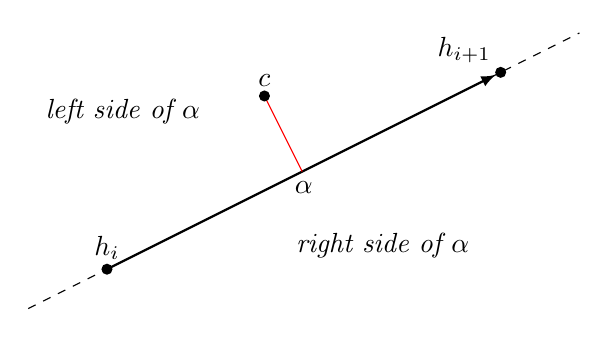
\begin{tikzpicture}
		\coordinate (HA) at (0, 0);
		\coordinate (HAL) at (-1,-0.5); 
		\coordinate (HB) at (5, 2.5);
		\coordinate (HBL) at (6, 3);
		\coordinate (P) at (2, 2.2);
		\coordinate (PINTERSECT) at (2.48,1.24);
			
		\fill (HA) circle (2pt) node[above] {$h_i$};
		\fill (HB) circle (2pt) node[above left] {$h_{i+1}$};
		%\fill (PINTERSECT) circle (2pt) node[above] {$a$};
		
		\draw[dashed] (HAL) -- (HBL);
		\draw[-latex, shorten >=2, thick] (HA) --node[below] {$\alpha$} (HB);
		\draw[red] (P) -- (PINTERSECT);
		\fill (P) circle (2pt) node[above] {$c$};

		\node at (0.2,2) {\textit{left side of $\alpha$}};
		\node at (3.5,0.3) {\textit{right side of $\alpha$}};
		
	\end{tikzpicture}
	\caption[short]{Representation of the concept of hyperplace, as well as \textit{left} and \textit{right} side of it.}
\end{figure}

Then if a point $c$ is on the \textit{left} side of all the edges in hull $H$, than $c$ is covered by $H$ (or inside $H$).

\begin{figure}[H]
	\centering
	\begin{tikzpicture}[scale=0.75]
		\coordinate (A) at (5, -4);
		\coordinate (B) at (14, 0);
		\coordinate (C) at (9, 4);
		\coordinate (D) at (1, -3);
		\coordinate (E) at (3, -1.7);
		\coordinate (F) at (5, 1.7);
		\coordinate (G) at (6, -2);
		\coordinate (H) at (8, 0);
		\coordinate (I) at (7, 3);
		\coordinate (J) at (2.7, 0.6);
		\coordinate (K) at (11, 1.4);
		\coordinate (L) at (9.4, -2.5);
		\coordinate (M) at (12, -2);
		\coordinate (N) at (2, 2.8);
		\coordinate (O) at (13, 2.6);
			
		\foreach \point in {A, B, C, D, E, F, G, H, I, J, K, L, M, N, O} {
			\fill (\point) circle (2pt);% node[above] {\point};
		}
		\foreach \s/\t in {A/M, M/B, B/O, O/C, C/N, N/D, D/A} {
			\draw[-latex, shorten >=2] (\s) -- (\t);
		}
	\end{tikzpicture}
	\caption[short]{Representation of a complete hull $H$, where every point $p \not \in H$ is to the left of all the edges of $H$}
\end{figure}

Aside from these structural specifics, this implementation deviates from the canonical one in some aspects.
First of all, the number of points added at each iteration is not fixed at one; instead, it is variable and falls within the interval $[1,|H|]$.
This choice is made purely for efficiency reasons.
Since each iteration requires computing the distance between each point and each edge of the pseudo-hull, why not add a point at each edge of the pseudo-hull?
It is easy to see that adding a point between one edge of the pseudo-hull does not interfere with adding points between other edges.
This approach saves computational power by avoiding the recomputation of values that are often the same at each iteration distance, while using more memory to store the list of candidates.

To further improve the performance of this sequential algorithm, a combination of SIMD instructions was used, specifically SSE and AVX instructions.
In some cases, this even resulted in doubling the overall performance.

\section{Parallhull}

In this section, the Parallhull algorithm will be introduced, describing the techniques and implementation strategies employed to optimize the computation of convex hulls through parallel processing.
The algorithm is based on a divide-and-conquer strategy where each processor will compute a convex hull on a different partition of the point set.
To find this local solution, the Quickhull implementation described above is employed.

\subsection{Merge Procedure}

The primary challenge in Parallhull was developing an efficient procedure to merge the convex hulls generated by each processor.
The objective is to merge the outputs from each CPU in pairs until only one solution remains.

A naive approach involves executing the Quickhull method on the union of all the points comprising the pair of convex hulls.
While this is correct, it can also be very inefficient.
Consider the worst case scenario for the Quickhull algorithm: each processor would start with $n/p$ points with a time complexity of the Quickhull in this scenario being $O((n/p)^2)$.
During the merging phase, Quickhull would need to process the entire set of $n$ points, resulting in $O(n\cdot log(n))$, as if the algorithm were running on the full set from the beginning.
This means that while the Quickhull algorithm can be effective as a merging procedure on average, it can also perform poorly in terms of efficiency in certain cases.

A more efficient approach leverages the representation of the hulls described in the previous section, as well as the properties of convex hulls in general.
Consider the merging of two hulls, $H_1$ and $H_2$ into $H_0$ and indicating with $h^i_j$ the j-th element in $H_i$.

This procedure begins by identifying the first element of $H_0$, $h^0_0$.
According to the way hulls are stored into the memory it is simple enough to set $h^0_0$ as the point that has the lowest $y$ coordinate between $h^1_0$ and $h^2_0$.

Then by moving along the both the hulls simultaneously and by making use of a gift-wrapping algorithm heavily specific to the merging of convex hull it is possible to merge two hulls with a time complexity of $O(|H_1|+|H_2|)$.
The ad-hoc gift-wrapping procedure is based on the same concepts explored when explaining the Quickhull method, particularly those related to the distance between a hull edge and a point, as well as the concepts of the \textit{left} and \textit{right} sides of an edge.
At each iteration, the goal is to determine which point between $H_1$ and $H_2$ should be kept in $H_0$.

For each $H_1$ and $H_2$ there is and index $j_k$, $k \in {1,2}$ that keeps track of the latest explored position in each hull.

Consider iteration $i$.
A candidate point must be selected, and often chosing the successor of $h^0_{i-1}$, denoted $h^s_{j_s-1}$, where $H_s$ is the hull from which $h^0_{i-1}$  was selected in the previous iteration, is a good choice.
Then, by the definition of convexity, $h^s_{j_s-1}$ is part of $H_0$ if there does not esists a point $p \in H_t$ where $H_t := {H_1, H_2} \backslash H_s$ such that $p$ is to the \textit{right} of hyperplane $\alpha$ generated from $(h^0_{i-1}, h^s_{j_s-1}$.
If point $p$ exists than the candidate is switched to $p$ and the computation performed again, with a careful procedure on which point of $H_s$ actually selecting if there is more than one point with the same properties as $p$.

The procedure as described does has a time complexity of $O(|H_1|^2+|H_2|^2)$ which means that, to reach time complexity of $O(|H_1|+|H_2|)$ there is still a small trick to use.
This trick consists in checking for the value obtained by plugging coordinates of the points in $H_t$ in the equation of the halfplane, obtaining a \textbf{pseudo-distance} value between point and hyperplane.
In fact one just need to check for the existance of $p$ while the value of this pseudo-distance between the halfplane and $h^t_k$ keeps increasing.
Once the pseudo-distance starts decreasing, by the property of hull convexity there are no points in $H_t$ that would pass through such hyperplane, thus stopping the search.

After designing and implementing this merge procedure it became evident that this is just an implementation of Chan's algorithm.
For the sake of simplicity this merging procedure will not be discussed more in depth in this paper.

\begin{figure}
	\centering
	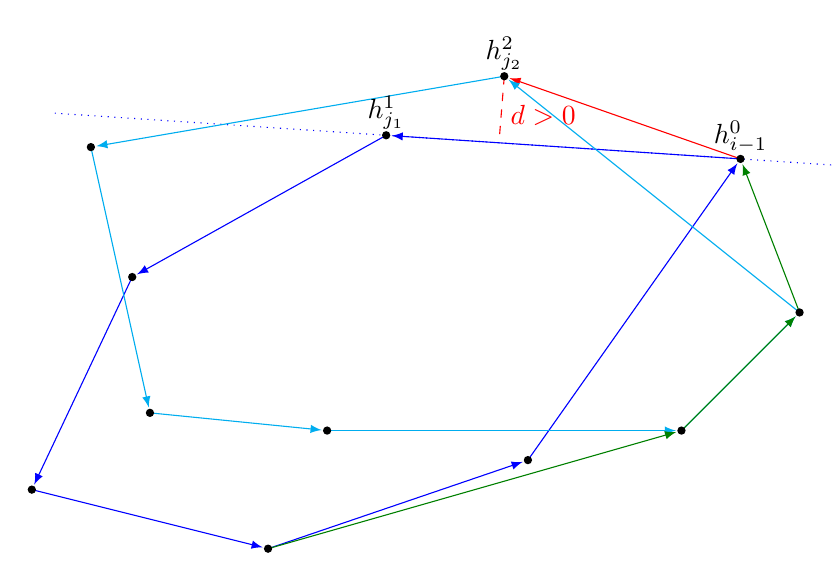
\begin{tikzpicture}[scale=0.75]
		\coordinate (A) at (5, -4);
		\coordinate (B) at (14, 0);
		\coordinate (C) at (9, 4);
		\coordinate (CL) at (8.88, 2.5);
		\coordinate (D) at (1, -3);
		\coordinate (E) at (3, -1.7);
		\coordinate (G) at (6, -2);
		\coordinate (H) at (13, 2.6);
		\coordinate (I) at (7, 3);
		\coordinate (J) at (2.7, 0.6);
		\coordinate (L) at (9.4, -2.5);
		\coordinate (M) at (12, -2);
		\coordinate (N) at (2, 2.8);
		
		\draw[dotted, blue, shorten <=-40, shorten >=-120] (H) -- (I);
		\draw[dashed, Red, shorten >=11] (C) -- node[right, shift={(0,0.07)}] {$d>0$} (CL);
		\draw[-latex, Red, shorten >=2] (H) --(C);
		
		%\fill (CL) circle (2pt) node[above] {CL};
		
		\foreach \s/\t in {A/L, L/H, H/I, I/J, J/D, D/A} {
			\draw[-latex, shorten >=2, blue] (\s) -- (\t);
		}
		\foreach \s/\t in {G/M, M/B, B/C, C/N, N/E, E/G} {
			\draw[-latex, shorten >=2, cyan] (\s) -- (\t);
		}
	
		\foreach \s/\t in {A/M, M/B, B/H} {
			\draw[-latex, shorten >=2, Green] (\s) -- (\t);
		}
		
		\foreach \point in {A, B, C, D, E, G, H, I, J, L, M, N} {
			\fill (\point) circle (2pt);% node[above] {\point};
		}	
	
		\node[above, shift={(0,-0.05)}] at (H) {$h^0_{i-1}$};
		\node[above, shift={(0,-0.05)}] at (I) {$h^1_{j_1}$};
		\node[above, shift={(0,-0.05)}] at (C) {$h^2_{j_2}$};
	
	\end{tikzpicture}
	\caption[short]{Example of merge between two hulls.}
\end{figure}

The merge procedure was implemented in multiple points in the final version of the project.
The most straightforward ones are the MPI implementation, in which different processes are launched toghether and share data according to OpenMPI specifications and the pthread implementations which relies on threads instead of processes.
The pthread version is a bit of a test made to check wheter using threads on a single CPU leads to some sort of performance gain over the MPI conterpart, but no major differences were noticed.

Finally the more complex application of the merging procedure happens when a single thread emulates the the multi-cpu code (which later will be refered to as \textit{Simulation}).

\section{Performance testing}

Performance tests were conducted on two different systems: a desktop computer and the Capri cluster.

\subsection{External factors}

While the tests themselves are straightforward, there are some unique time characteristics to be aware of.
One such consideration is the time required for OpenMPI to initialize, which usually takes a bit more than a second.
Another important time-related factor is the time required to read the file containing the set of points or to generate the set of points itself.
% From a computational perspective, a very big number of point is required to obtain results of some value and reading them as raw values is the fastest way to process them, rather than creating them with a random generation procedure at each run.

Additionally, the way the point set is generated can significantly impact the execution time.
In fact, the performance of the Quickhull algorithm improves when the points are arranged in a cloud with a higher density toward the center.
In order to obtain somewhat balanced results, each set of points used to obtain the results of the following graphs was generated as a uniform distribution of points inside a circle.

Other minor factors that slightly affect performance are related to hardware, such as differences in clock speed between processors, power limits, thermal limits, and so on.

\subsection{Main results}

This section will present the raw results obtained by selecting the best of two successive executions for each parameters configuration.
The same criterion of conducting at least two runs for each configuration was used while gathering the data presented in this paper.

\begin{figure}[H]
    \centering
    \begin{tikzpicture}
        \begin{axis}[
            width=12cm, height=8cm,
			xmajorgrids=true,
            ymajorgrids=true,
            grid style={dashed,gray!30},
            xlabel=CPUs,
            ylabel=time(s),
            xtick=data,
            %ytick={2,3,4,5,6,7,8,9},
			xmin=0,ymin=0,
            ]
			\addplot[color=Blue,mark=square,] coordinates {(1,8.91)(2,5.12)(3,4.03)(4,3.46)(5,3.08)(6,2.88)(7,2.74)(8,2.67)};
        \end{axis}
    \end{tikzpicture}
    \caption{Execution time of the Parallhull algorithm without considering initialization costs on a Capri using a point set of $10^9$ points. Lower is better} \label{fig:fullTimeGraph}
\end{figure}

\begin{figure}[H]
    \centering
    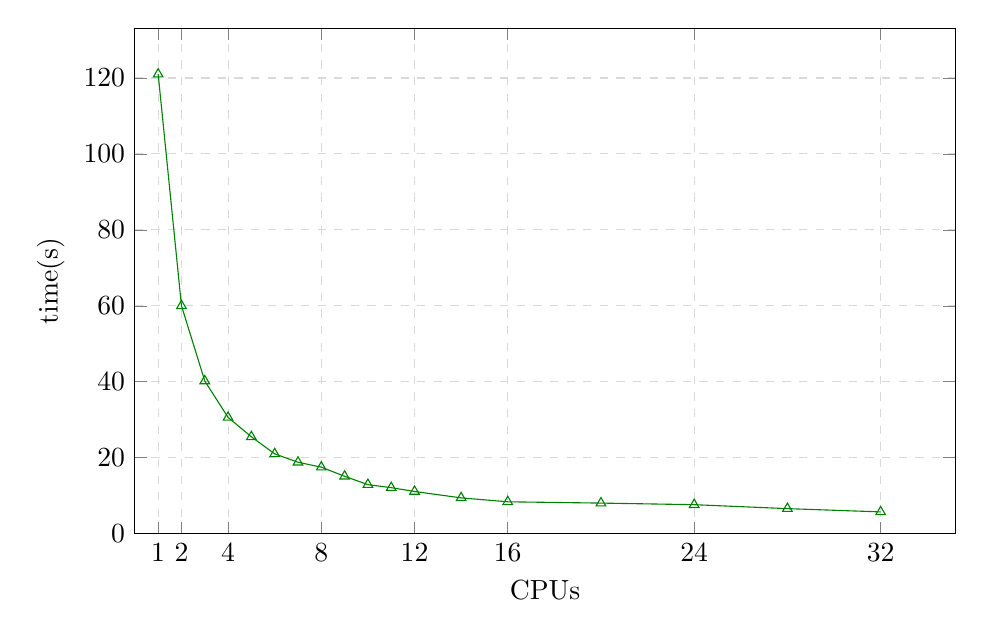
\begin{tikzpicture}
        \begin{axis}[
            width=12cm, height=8cm,
            ymajorgrids=true,
			xmajorgrids=true,
            grid style={dashed,gray!30},
            xlabel=CPUs,
            ylabel=time(s),
            xtick={1, 2, 4, 8, 12, 16, 24, 32},
            %ytick={120,60,30,15,5},
			xmin=0,ymin=0,
            ]
			\addplot[color=Green,mark=triangle,] coordinates {(1,121)(2,60)(3,40.2)(4,30.6)(5,25.5)(6,21)(7,18.8)(8,17.5)(9,15.1)(10,12.9)(11,12.1)(12,11.1)(14,9.41)(16,8.38)(20,8.04)(24,7.62)(28,6.58)(32,5.72)};

        \end{axis}
    \end{tikzpicture}
    \caption{Execution time of the Parallhull algorithm without considering initialization costs on a desktop PC using a point set of $5 \cdot 10^9$ points. Lower is better}
\end{figure}

\begin{figure}[H]
	\centering
	\begin{tabular}{|c | c | c|} 
		\hline
		Number of CPUs & Execution time(Desktop) & Execution time (Capri) \\ [0.5ex] 
		\hline%\hline
		1 & 8.91 & 121 \\ 
		\hline
		2 & 5.12 & 60.0 \\
		\hline
		3 & 4.03 & 40.2 \\
		\hline
		4 & 3.46 & 30.6 \\
		\hline
		5 & 3.08 & 25.5 \\
		\hline
		6 & 2.88 & 21.0 \\
		\hline
		7 & 2.74 & 18.8 \\
		\hline
		8 & 2.67 & 17.5 \\
		\hline
		9 & - & 15.1 \\
		\hline
		10 & - & 12.9 \\
		\hline
		11 & - & 12.1 \\
		\hline
		12 & - & 11.1 \\
		\hline
		14 & - & 9.41 \\
		\hline
		16 & - & 8.38 \\
		\hline
		20 & - & 8.04 \\
		\hline
		24 & - & 7.62 \\
		\hline
		28 & - & 6.58 \\
		\hline
		32 & - & 5.72 \\
		\hline
	\end{tabular}
	\caption{Execution times without initialization time. Each value is the lowest between two acquisitions with the same settings.}
\end{figure}

\subsubsection{Speedup \& Scalability}

While the graphs and table above show the actual time taken for each configuration, this section will discuss the speedup and the scalability achieved by each configuration.
Since the execution times gathered do not include the fixed costs time either from OpenMPI or from the file reading, which is considered initialization, the graphs for the speedup and the scalability are effectively the same.

\begin{figure}[H]
    \centering
    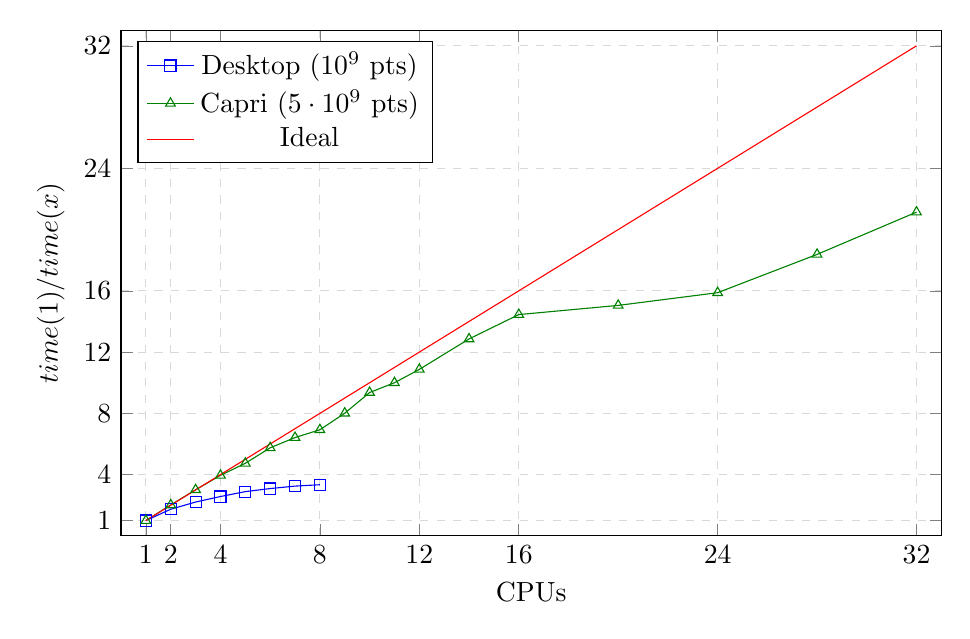
\begin{tikzpicture}
        \begin{axis}[
            width=12cm, height=8cm,
            ymajorgrids=true,
			xmajorgrids=true,
            grid style={dashed,gray!30},
            xlabel=CPUs,
            ylabel=$time(1)/time(x)$,
            legend style={at={(0.02,0.98)},anchor=north west,},
            xtick={1, 2, 4, 8, 12, 16, 24, 32},
            ytick={1, 4, 8, 12, 16, 24, 32},
			xmin=0,ymin=0,xmax=33,ymax=33
            ]
			\addplot[color=Blue,mark=square,] coordinates {(1,1)(2,1.74)(3,2.21)(4,2.57)(5,2.89)(6,3.09)(7,3.25)(8,3.34)};
			\addplot[color=Green,mark=triangle,] coordinates {(1,1)(2,2.02)(3,3.01)(4,3.95)(5,4.74)(6,5.75)(7,6.42)(8,6.93)(9,8.01)(10,9.36)(11,10)(12,10.87)(14,12.86)(16,14.45)(20,15.05)(24,15.88)(28,18.38)(32,21.14)};
			\addplot[color=Red,] coordinates {(1,1)(2,2)(3,3)(4,4)(5,5)(6,6)(7,7)(8,8)(9,9)(10,10)(11,11)(12,12)(14,14)(16,16)(20,20)(24,24)(28,28)(32,32)};
            \legend{Desktop ($10^9$ pts), Capri ($5 \cdot 10^9$ pts), Ideal}
        \end{axis}
    \end{tikzpicture}
    \caption{Higher is better.} \label{fig:speedupZoom}
\end{figure}

As \figurename{ \ref{fig:fullTimeGraph}} shows, the speedup on the Capri cluster is close to, if not optimal.
Scalability on the other end seems to suffer a decrease in efficiency strating from the 16 CPUs mark.
This is likely due to Capri's harware resources since it is composed of four nodes each containing a four CPUs with 16 cores each.
A likely explaination would be that all processes were executed on a single CPU, or at least a single node, up until more than 16 tasks were launched, which means that the slowdown should be caused by communication latency.

\begin{figure}[H]
    \centering
    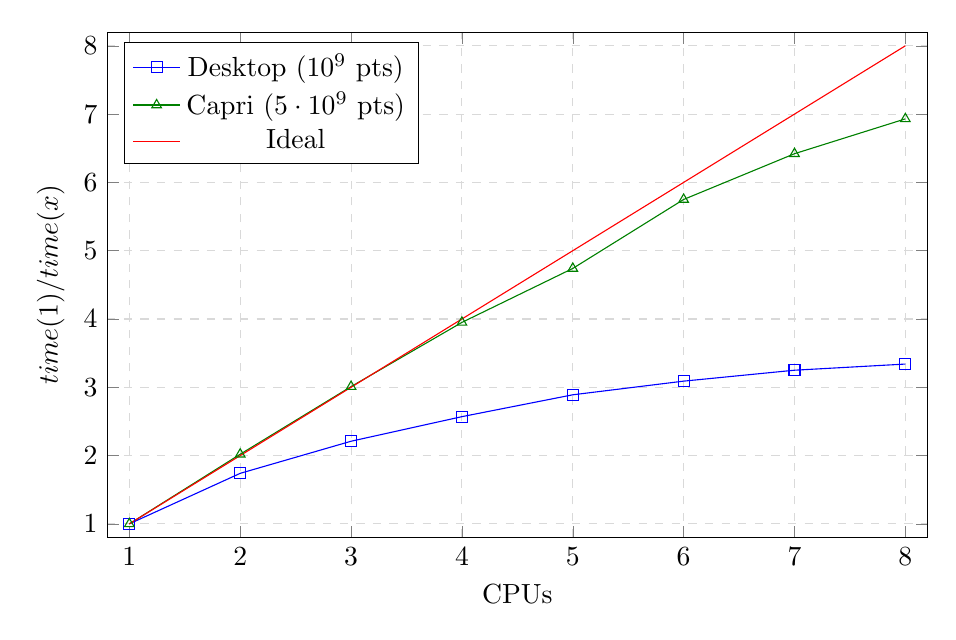
\begin{tikzpicture}
        \begin{axis}[
            width=12cm, height=8cm,
            ymajorgrids=true,
			xmajorgrids=true,
            grid style={dashed,gray!30},
            xlabel=CPUs,
            ylabel=$time(1)/time(x)$,
            legend style={at={(0.02,0.98)},anchor=north west,},
            xtick={1, 2, 3, 4, 5, 6, 7, 8},
            ytick={1, 2, 3, 4, 5, 6, 7, 8},
			xmin=0.8,ymin=0.8,xmax=8.2,ymax=8.2
            ]
			\addplot[color=Blue,mark=square,] coordinates {(1,1)(2,1.74)(3,2.21)(4,2.57)(5,2.89)(6,3.09)(7,3.25)(8,3.34)};
			\addplot[color=Green,mark=triangle,] coordinates {(1,1)(2,2.02)(3,3.01)(4,3.95)(5,4.74)(6,5.75)(7,6.42)(8,6.93)};
			\addplot[color=Red,] coordinates {(1,1)(2,2)(3,3)(4,4)(5,5)(6,6)(7,7)(8,8)};
            \legend{Desktop ($10^9$ pts), Capri ($5 \cdot 10^9$ pts), Ideal}
        \end{axis}
    \end{tikzpicture}
    \caption{Zoom on the previous graph with focus on the $[0,8]$ range. Higher is better.}
\end{figure}

The curves are generally as expected: for the most part, the measured $time(1)/time(x)$ is below the ideal line, which represents a linear 1:1 ratio.
However, upon closer inspection, there are some anomalies.
In Capri's measurements, the speedup with 2 and 3 CPUs exceeded the ideal speedup value.
Specifically, the values were $time(2) = 2.02$ and $time(3) = 3.01$.

While this phenomenon could be attributed to the \textit{acquisition of bad data}, it's possible that the single CPU run was affected by external factors, such as the simultaneous execution of multiple programs on the same machine.
However, given the specifics of the problem, this is unlikely to be the case.

\subsubsection{Simulation testing} \label{section:simul}

The most likely reason for this behavior is more plausibly connected to the structure of the algorithm.
To explain this, let's introduce a sort of \textbf{simulation} of parallel execution with multiple CPUs on a single CPU.
This approach was developed in the early stages of the project to provide a more controlled environment for testing and debugging the merging procedure, without having to worry about synchronization and communication issues.

This simulation is controlled by setting an upper bound on the number of points that Quickhull can process.
This means that when the number of points in the input set exceeds the upper bound, the input set will be split into smaller subsets to adhere to the Quickhull upper bound, effectively creating $s = \lceil (|N|/ub) \rceil$ subproblems.
the subproblems are then solved sequentially, one after the other, and are merged two at a time after all subproblems have been solved.

Using the same set of $10^9$ elements uniformly distributed within a circle as the input set on the desktop machine, various values for the upper bound were tested.

\begin{figure}[H]
    \centering
    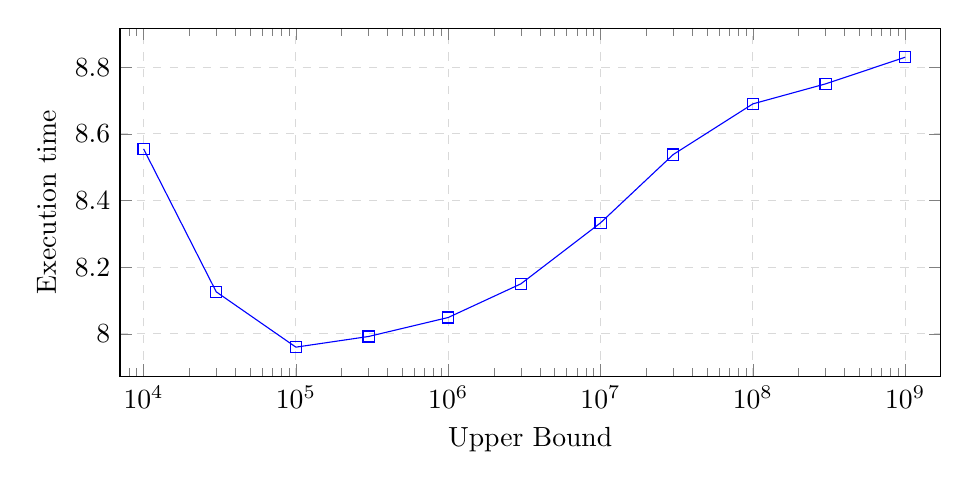
\begin{tikzpicture}
        \begin{axis}[
            width=12cm, height=6cm,
			xmode=log,
            ymajorgrids=true,
			xmajorgrids=true,
            grid style={dashed,gray!30},
            xlabel=Upper Bound,
            ylabel=Execution time,
			xmin=7e3,xmax=17e8,
            ]
			\addplot[color=Blue,mark=square,] coordinates {(1e9,8.83)(3e8,8.75)(1e8,8.69)(3e7,8.538)(1e7,8.333)(3e6,8.15)(1e6,8.049)(3e5,7.992)(1e5,7.96)(3e4,8.126)(1e4,8.555)};
        \end{axis}
    \end{tikzpicture}
    \caption{Execution time on a single CPU in function of the upper bound.}
\end{figure}

\begin{figure}[H]
    \centering
    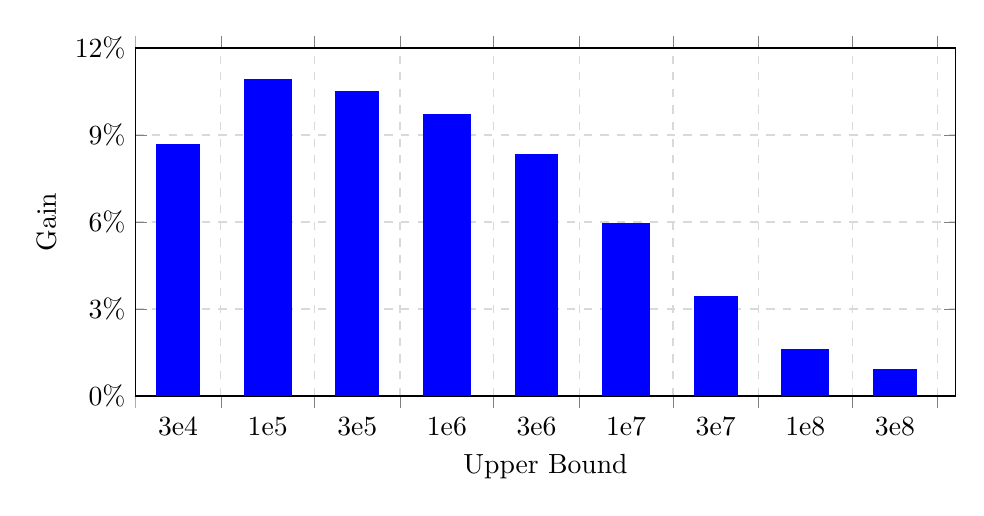
\begin{tikzpicture}
        \begin{axis}[
            width=12cm, height=6cm,
			xmode=log,
            ymajorgrids=true,
			xmajorgrids=true,
            grid style={dashed,gray!30},
            xlabel=Upper Bound,
            ylabel=Gain,
            xtick={3e8,1e8,3e7,1e7,3e6,1e6,3e5,1e5,3e4,1e4},
            xticklabels={3e8,1e8,3e7,1e7,3e6,1e6,3e5,1e5,3e4,1e4},
            ytick={0,3,6,9,12},
			yticklabels={0\%, 3\%, 6\%, 9\%, 12\%},
			ybar interval=0.5,
			ymin=0,ymax=12,xmin=1e4,xmax=378107170,
            ]
			\addplot[color=Blue,fill] coordinates {(3e8,0.91)(1e8,1.61)(3e7,3.42)(1e7,5.96)(3e6,8.34)(1e6,9.7)(3e5,10.49)(1e5,10.93)(3e4,8.66)(1e4,3.21)};
        \end{axis}
    \end{tikzpicture}
    \caption{Gained percentage over no upper bound.}
\end{figure}

As the graphs above show, the gain achieved by setting an appropriate upper bound is significant.
However, this behavior raises some questions: why exactly does it happen?
A definitive answer may require conducting additional experiments and adjusting the code, but since this topic is outside the scope of this project, only speculative comments can be provided.

\begin{itemize}
	\item The implementation of the Quickhull algorithm is not optimal; therefore, when dealing with a large number of points, its inefficiency becomes evident.
	\item This behavior appears only with this specific distribution of points: it's possible that, toward the final iterations of Quickhull, the remaining points are all positioned around the edge, causing Quickhull to perform as a worst-case scenario (at least in the last iterations).
	\item There is indeed a correlation and an optimal value for the upper bound that balances the number of subproblems to achieve the best performance.
\end{itemize}

\section{Conclusion}

Parallhull is an algorithm that performs very well indeed, especially when working with large amount of data (as most parallel algorithms do).
The speedup it provided on the Capri cluster can be considered very close to optimal.
%Capri is not a private resource and therefore it is subseptible to external factors, like scheduling of other users's running jobs.

Scalability instead can be subject of debate: as shown by \figurename{ \ref{fig:speedupZoom}} the speedup is optimal when using a small amount of CPUs, while it gets worse as the number of CPUs increases, especially above the 16 CPUs mark.
This is an expected behavior and could be caused by external factors like the uneven load of the nodes in the cluster.

As shown in Section \ref{section:simul}, splitting the problem into more subproblems improves performance, even when execution occurs on a single CPU, with gains that can reach double-digit figures.
Based on this concept, it is possible to hypothesize that the calculated speedup value may not reflect the true speedup.
The key point is that the benefits of dividing the problem into subproblems were not accounted for.
This means that both the speedup as well as scalability deductions made in this paper are likely optimistic ones.

To resolve this theoretical discrepancy, an upper bound must be established so that, regardless of the number of CPUs used, the number of problems solved remains constant.
To define such upperbound one should test multiple values on different input set distributions and even shuffle them at the beginning to diversify the content of each partition.
Testing using different sizes for the input set is also a good practice to avoid overfitting.

% \begin{thebibliography}{9}

% \end{thebibliography}

\end{document}

